% !TeX root = tcolorbox.tex
% include file of tcolorbox.tex (manual of the LaTeX package tcolorbox)
\clearpage
\section{Initialization Option Keys}\label{sec:initkeys}%
\tcbset{external/prefix=external/initoptions_}%
The \emph{initialization} options are only applicable for the generation
of new environments and commands based on |tcolorbox| and friends.
Particularly, they can be used for
\begin{itemize}
\item\refCom{newtcolorbox},
\item\refCom{newtcbox},
\item\refCom{newtcblisting},
\item\refCom{newtcbinputlisting},
\item\refCom{newtcbtheorem}, and
\item\refCom{newtcboxfit}.
\end{itemize}

\bigskip
\begin{marker}
Typically, these options may generate counters and alike.
It is \textbf{strongly} recommended that you use initialization options inside
the preamble only. Otherwise, you may get trouble when using \LaTeX's |\include| features.
\end{marker}


\subsection{Numbered Boxes}\label{sec:numberedboxes}
Counters assigned using the initialization options are administrated
automatically. Especially, they are increased for each new box.
Independent from the real counter name, the counter value can be
referenced by \docAuxCommand{thetcbcounter}, e.\,g.\ inside the title of
the box. The real counter name is stored inside \docAuxCommand{tcbcounter}.

\begin{newTcbKey}{auto counter}{}{no value, initially unset}
Creates a new counter automatically.
With \refKey{/tcb/new/number format} and
\refKey{/tcb/new/number within}, the appearance and behavior of the counter
can be changed. The counter value is referenced by \docAuxCommand{thetcbcounter}.

\inputpreamblelisting{A}

\begin{dispExample}
\begin{pabox}[label={myautocounter}]{Title with number}
This box is automatically numbered with \ref{myautocounter} on page
\pageref{myautocounter}. Inside the box, the \thetcbcounter\ can
also be referenced by |\thetcbcounter|.
The real counter name is \texttt{\tcbcounter}.
\end{pabox}
\end{dispExample}
\end{newTcbKey}

\clearpage
\begin{newTcbKey}{use counter from}{=\meta{tcolorbox}}{no default, initially unset}
Here, a counter from another \meta{tcolorbox} is reused.
Note that the settings for \refKey{/tcb/new/number format} and
\refKey{/tcb/new/number within} are inherited and cannot be changed.
The counter value is referenced by \docAuxCommand{thetcbcounter}.

\begin{dispExample}
\newtcolorbox[use counter from=pabox]{mybox}[2][]{%
colback=blue!5!white,colframe=blue!75!black,fonttitle=\bfseries,
title=Some Box \thetcbcounter: #2,#1}

\begin{mybox}[label={myusecounterfrom}]{Title with continued number}
This box is automatically numbered with \ref{myusecounterfrom} on page
\pageref{myusecounterfrom}. Inside the box, the \thetcbcounter\ can
also be referenced by |\thetcbcounter|.
The real counter name is \texttt{\tcbcounter}.
\end{mybox}
\end{dispExample}
\end{newTcbKey}


\begin{newTcbKey}{use counter}{=\meta{counter}}{no default, initially unset}
Here, an ordinary existing \LaTeX\ \meta{counter} is used for numbering.
With \refKey{/tcb/new/number format} and
\refKey{/tcb/new/number within}, the appearance and behavior of the counter
can be changed. The counter value is referenced by \docAuxCommand{thetcbcounter}.

\begin{dispExample}
% \newcounter{myexample}%  preamble
\newtcolorbox[use counter=myexample,number format=\Alph]{mybox}[2][]{%
colback=green!5!white,colframe=green!55!black,fonttitle=\bfseries,
title=Some Box \thetcbcounter: #2,#1}

\begin{mybox}[label={myusecounter}]{Title with \LaTeX\ number}
This box is automatically numbered with \ref{myusecounter} on page
\pageref{myusecounter}. Inside the box, the \thetcbcounter\ can
also be referenced by |\thetcbcounter|.
The real counter name is \texttt{\tcbcounter}.
\end{mybox}
\end{dispExample}
\end{newTcbKey}


\begin{newTcbKey}[][doc new=2014-09-19]{use counter*}{=\meta{counter}}{no default, initially unset}
An existing \LaTeX\ \meta{counter} is used for numbering. In contrast to
\refKey{/tcb/new/use counter}, the options \refKey{/tcb/new/number format} and
\refKey{/tcb/new/number within} are ignored. Use this for counters which
are already configured outside the |tcolorbox| package, e.\,g.\ the standard
|figure| counter.
\end{newTcbKey}


\begin{newTcbKey}{no counter}{}{no value, initially set}
The created boxes are not numbered. This is the default. The option may
be used to overrule a previous option.
\end{newTcbKey}

\enlargethispage*{1cm}

\begin{newTcbKey}[][doc new=2019-10-18]{reset counter on overlays}{\colOpt{=true\textbar false}}{default |true|, initially |false|}
For |beamer| slides, this invokes the |\resetcounteronoverlays| command
for the box counter. The counter is automatically reset on subsequent
overlay slides of a frame.
Thereby, the counter will be the same on all slides of every frame.
\end{newTcbKey}


\clearpage
\begin{newTcbKey}{number within}{=\meta{counter}}{no default, initially unset}
The automatic counter is set to zero, if \meta{counter} is increased.
Additionally, during output, the value of \meta{counter} is prepended to the value of
the automatic counter.\par
To prepend the automatic counter with the chapter number and to reset it
with every new chapter, use:
\begin{dispListing}
number within=chapter
\end{dispListing}
See \refKey{/tcb/new/use counter} for a complete example.
\end{newTcbKey}


\begin{newTcbKey}{number format}{=\meta{format macro}}{no default, initially \texttt{\textbackslash arabic}}
Declares the format of the automatic counter. The \meta{format macro} can be
any valid \LaTeX\ number formatting macro like |\arabic|, |\roman|, etc.\par
To display the counter value in large roman numbers, use:
\begin{dispListing}
number format=\Roman
\end{dispListing}
See \refKey{/tcb/new/auto counter} for a complete example.
\end{newTcbKey}


\begin{newTcbKey}{number freestyle}{=\meta{code}}{no default, initially unset}
Allows advanced control over the complete number format. This option overrules
the format given by \refKey{/tcb/new/number within} and \refKey{/tcb/new/number format}.
Nevertheless, you can combine it with \refKey{/tcb/new/number within} to
get the desired reset property.\par
The \meta{code} is some formatting code which should contain |\tcbcounter| to
reference the automated counter. Since this \meta{code} is expanded, you have
to secure each macro with |\noexpand| with \emph{exception} of |\tcbcounter|.

\inputpreamblelisting{H}

\begin{dispExample}
\begin{phbox}[label={myfreestyle}]{Title with freestyle number}
This box is automatically numbered with \ref{myfreestyle} on page
\pageref{myfreestyle}. Inside the box, the \thetcbcounter\ can
also be referenced by |\thetcbcounter|.
The real counter name is \texttt{\tcbcounter}.
\end{phbox}
\end{dispExample}
\end{newTcbKey}

\clearpage
\begin{marker}
The following options \refKey{/tcb/new/crefname} and \refKey{/tcb/new/Crefname}
need to be set inside the preamble.
\end{marker}

\begin{newTcbKey}[][doc updated=2014-12-01]{crefname}{=\marg{singular}\marg{plural}}{no default, initially unset}
  This option key can be used only in conjunction with the |cleveref| package
  \cite{cubitt:2018a} which has to be loaded separately.
  It creates a cross-reference type for the new |tcolorbox|'es, where the
  lowercase \meta{singular} and \meta{plural} forms of the cross-reference are given.
  This type is the environment or macro name and \refKey{/tcb/label type} is set automatically.
  See \refKey{/tcb/label type} and \cite{cubitt:2018a} for more information.
\end{newTcbKey}


\begin{newTcbKey}[][doc updated=2014-12-01]{Crefname}{=\marg{singular}\marg{plural}}{no default, initially unset}
  This option key can be used only in conjunction with the |cleveref| package
  \cite{cubitt:2018a} which has to be loaded separately.
  It creates a cross-reference type for the new |tcolorbox|'es, where the
  uppercase \meta{singular} and \meta{plural} forms of the cross-reference are given.
  This type is the environment or macro name and \refKey{/tcb/label type} is set automatically.
  See \refKey{/tcb/label type} and \cite{cubitt:2018a} for more information.
\end{newTcbKey}

\inputpreamblelisting{I}
\begin{dispExample}
% \usepackage{varioref}
% \usepackage{cleveref}
\begin{mybluebox}[label={myreference}]{My title}
This is an example.
\end{mybluebox}

\Cref{myreference}, \cref{myreference}.\\
\Cpageref{myreference}, \cpageref{myreference}.\\
\nameCref{myreference}, \namecref{myreference}.\\
\labelcref{myreference}, \labelcpageref{myreference}.\\
With \texttt{varioref}:\\
\Vref{myreference}, \vref{myreference}.\\
\Vref*{myreference}, \vref*{myreference}.
\end{dispExample}

\clearpage

\begin{newTcbKey}[][doc new=2014-09-19]{blend into}{=\meta{name}}{style, no default, initially unset}
Used to comfortably blend into an existing schema of naming and numbering for
some selected cases. For example, a |tcolorbox| can be used to display
and entitle an image pretending to be a standard |figure| environment.
Here, \refKey{/tcb/title} is used instead of the standard |\caption|
and \refKey{/tcb/list text} can be used instead of the optional parameter
of the standard |\caption|.

Feasible values for \meta{name} are:
\begin{itemize}
\item\docValue{figures}: blend into the standard |figure| environment.
\item\docValue{tables}: blend into the standard |table| environment.
\item\docValue{listings}: blend into the standard |lstlisting| environment
  of the package |listings| \cite{hoffmann:listings}.
  \begin{marker}
  Note that |blend into=listings| can only be used in the document content
  or, preferably, inside a |\AtBeginDocument| clause! Using it without
  |\AtBeginDocument| inside the preamble does not work since the |listings|
  packages initializes its counter also inside |\AtBeginDocument|.
  \end{marker}
\end{itemize}
\end{newTcbKey}

\enlargethispage*{5cm}
\begin{dispListing}
\begin{figure}[htb]
  \centering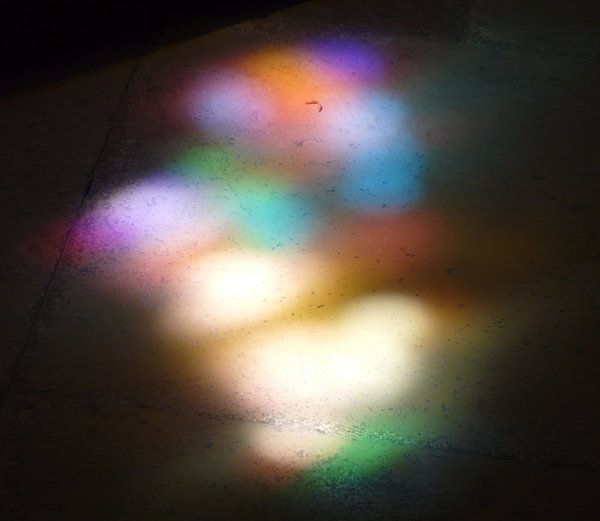
\includegraphics[height=4cm]{lichtspiel.jpg}
  \caption{A standard figure}
\end{figure}

\newtcolorbox[blend into=figures]{myfigure}[2][]{float=htb,capture=hbox,
  title={#2},every float=\centering,#1}

\begin{myfigure}{A tcolorbox figure}
  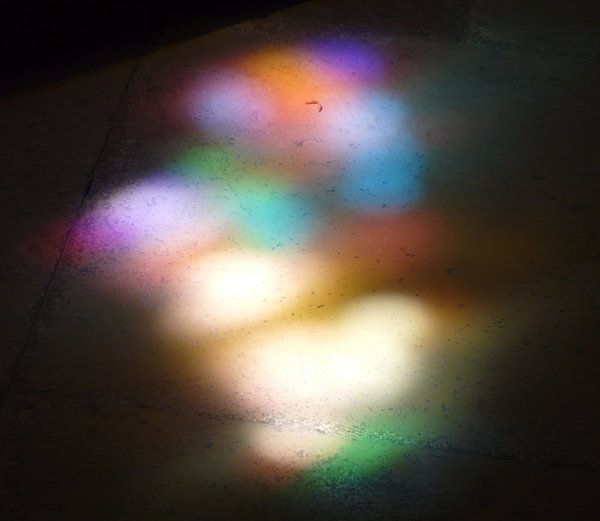
\includegraphics[height=4cm]{lichtspiel.jpg}
\end{myfigure}
\end{dispListing}
{\tcbusetemp}



\clearpage
\begin{docTcbKey}[][doc new=2015-03-13]{blend before title}{=\meta{value}}{no default, initially \docValue{colon}}
  This option formats the title output of \refKey{/tcb/new/blend into}.
  Note that this is a common |tcolorbox| option which should be set
  globally or in the normal option part of \refCom{newtcolorbox}.

Feasible values for \meta{value} are:
\begin{itemize}
\item\docValue{colon}: use name/number plus colon.
\item\docValue{dash}: use name/number plus dash.
\item\docValue{colon hang}: use name/number plus colon with hanging indent.
\item\docValue{dash hang}: use name/number plus dash with hanging indent.
\end{itemize}

\begin{dispListing}
\newtcolorbox[blend into=figures]{myfigure}[2][]{float=htb,capture=hbox,
  blend before title=dash hang,title={#2},every float=\centering,#1}

\begin{myfigure}{A tcolorbox figure with quite a long title}
  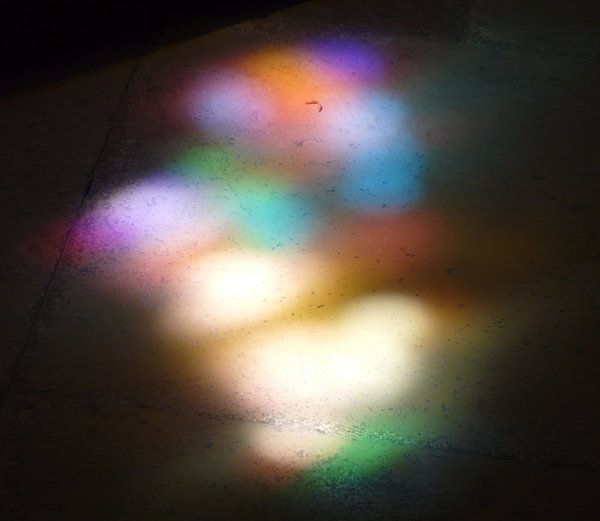
\includegraphics[height=5cm]{lichtspiel.jpg}
\end{myfigure}
\end{dispListing}
{\tcbusetemp}
\end{docTcbKey}

\clearpage
\begin{docTcbKey}[][doc new=2015-03-13]{blend before title code}{=\meta{code}}{no default}
  This option formats the title output of \refKey{/tcb/new/blend into}.
  The \meta{code} takes one parameter, the name/number.
  Use this, if \refKey{/tcb/blend before title} is not flexible enough.

\begin{dispListing}
\newtcolorbox[blend into=figures]{myfigure}[2][]{float=htb,capture=hbox,
  blend before title code={\fbox{##1}\ },title={#2},every float=\centering,#1}

\begin{myfigure}{A tcolorbox figure}
  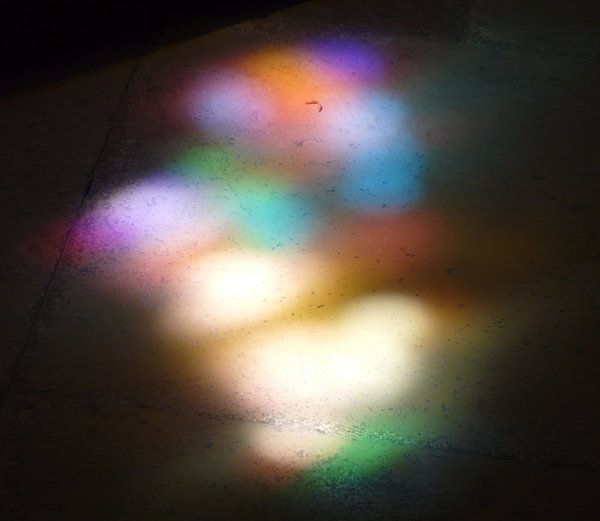
\includegraphics[height=6cm]{lichtspiel.jpg}
\end{myfigure}
\end{dispListing}
{\tcbusetemp}
\end{docTcbKey}



\clearpage
\subsection{Lists of \texttt{tcolorbox}es}\label{sec:listsof}
For figures and tables, \LaTeX\ provides the |\listoffigures| and
|\listoftables| commands to create lists of these numbered entities.
Also, a |tcolorbox| can be part of such a kind of list.
\begin{enumerate}
\item Assign a list \meta{name} by the \emph{initialization} option
  \refKey{/tcb/new/list inside}.
\item Optionally, a new \meta{type} for list entries may be assigned
  by the \emph{initialization} option \refKey{/tcb/new/list type}.
\item List entries a generated automatically within each new |tcolorbox|
  using the above initialization.
  \begin{itemize}
  \item If \refKey{/tcb/list entry} is set, the entry is generated with it.
  \item Otherwise, if \refKey{/tcb/title} is set, the entry is generated with it.
  \item Otherwise, the entry is generated with the current number and the environment name.
  \end{itemize}
\item The generated list is displayed by \refCom{tcblistof}.
\end{enumerate}

\begin{newTcbKey}{list inside}{=\meta{name}}{no default, initially unset}
Assigns a list or contents file to the generated |tcolorbox|es.
Entries to this list are saved to a file which gets the \meta{name} as
file name extension. The list is referenced by this name in
\refCom{tcblistof}.
For example:
\begin{dispListing}
list inside=exam
\end{dispListing}
See Section \ref{listing:exercises} from page \pageref{listing:exercises}
for a complete example.
\end{newTcbKey}


\begin{newTcbKey}{list type}{=\meta{type}}{no default, initially |tcolorbox|}
Optionally, some \meta{type} can be assigned to the list entries.
For a new \meta{type}, a macro |\l@|\meta{type} has to exist which controls
the format of the list entry. The default type is defined by
\begin{dispListing}
\newcommand*\l@tcolorbox{\@dottedtocline{1}{1.5em}{2.3em}}
\end{dispListing}
This is identical to the |\l@section| setting of \LaTeX. |\l@tcolorbox| can
be redefined or a new \meta{type} can be assigned.
\end{newTcbKey}


\begin{docCommand}{tcblistof}{\oarg{macro}\marg{name}\marg{title text}}
Displays the generated list of |tcolorbox|es with the given \meta{name}.
The heading is generated by \meta{macro}\marg{title text} where \texttt{\textbackslash section}
is the default setting for \meta{macro}.\par
To display the list inside a subsection, use for example:
\begin{dispListing}
\tcblistof[\subsection]{exam}{List of Exercises}
\end{dispListing}
The result of the example is found as Subsection \ref{listofexercises} on
page \pageref{listofexercises}.
\begin{marker}
The core of the list is generated by |\@starttoc|\marg{name} which
can be wrapped into an own macro.
\end{marker}
\end{docCommand}

